For each of the three outcomes, the target causal parameter is the Average Treatment Effect, which is the difference in the expected counterfactual if all recruited students had taken the entrepreneurial training and the expected counterfactual if none of the students were assigned to the treatment.

\[ \Psi^{\mathcal{F}}(\mathbb{P}_{U,X}) = \mathbb{E}_{U,X}(Y_1) - \mathbb{E}_{U,X}(Y_0)  \]

Because of the design of the experiment as an RCT (randomized control trial), we can conclude that $A$ is a function of $U_A$ only, so that there must be an exclusion restriction between $W$ and $A$. See p. 24 of \cite{tlb} for confirmation of this claim. A second consequence of our randomizing the intervention node $A$ is that we may assume that $U_A$ is independent of $U_Y$ and of $U_W$. We can test this assumption for $U_A$ and $U_W$ by using a balance table. There is no way for us to test the independence assumption of $U_A$ and $U_Y$. This corresponds to believing that there are no unmeasured factors that predict both $A$ and the outcome $Y$, which is often called the no unmeasured confounders assumption. This independence assumption also means that there is no backdoor path from $Y$ to $A$. Therefore our causal estimand is identifiable from the statistical estimand. Our structural causal assumes that the observed data were generated by the following actions: \\

\begin{enumerate}
\item Drawing unobservable $U=(U_A, U_Y, U_W)$ from some probability distribution $\probability_U$ ensuring that $U_A$ is independent of $U_Y$, given $W$.
\item Generating $W$ as a deterministic function of $U_W$.
\item Generating $A$ as a deterministic function of $W$ and $U_A$.
\item Generating $Y$ as a deterministic function of $W$, $A$, and $U_Y$.
\end{enumerate} 

The time ordering of the variables is $W \to A \to Y$, while for the causal ordering, both $W$ and $A$ precede $Y$, and neither $W$ nor $A$ precede each other. This model is illustrated in the figure \ref{fig:DAG}. Note that there are no assumptions on functional forms in our model. Nevertheless, because of the randomization of $U_A$ via a random number generator with a specified distribution, our model is technically speaking only semi-parametric, and not completely non-parametric.\\

\begin{figure}[h]
  \centering
  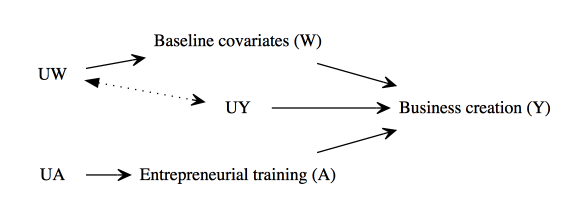
\includegraphics{../../DAG_Uganda.png}
  \caption{Figure 1: Structural causal model\label{fig:DAG}}
\end{figure}


%%% Local Variables:
%%% mode: latex
%%% TeX-master: "../main/report"
%%% End:
